\documentclass[10pt]{article}
\usepackage[a4paper,margin=1.6cm,top=1.3cm,bottom=1.3cm]{geometry}
\usepackage[T1]{fontenc}
\usepackage{lmodern}
\usepackage{microtype}
\usepackage{booktabs}
\usepackage{graphicx}
\usepackage{enumitem}
\usepackage{xcolor}
\usepackage[colorlinks=true,linkcolor=black,citecolor=black,urlcolor=blue]{hyperref}
\setlist{nosep,leftmargin=1.2em,topsep=1pt}
\setlength{\parindent}{0pt}
\setlength{\parskip}{3pt}
\pagestyle{empty}
\newcommand{\head}[1]{\par\smallskip{\large\bfseries #1}\par}
\newcommand{\sect}[1]{\par\smallskip{\bfseries\color{black!80} #1}\par}

\begin{document}
\head{Idea 10 PoC --- The disposition effect and earnings news in China}
\textit{Proof of concept, October 2026. Code: \texttt{idea10\_disposition\_cgo/run.py}.}

\sect{Question and design}
Frazzini (2006) shows that US post-earnings drift is strongest when the news and the shareholders' unrealised
capital gains share a sign. Disposition-prone holders sell winners into good news and hold losers through bad news,
which slows price adjustment. China's retail-heavy, high-turnover market is a natural setting, and we found no
direct test. The capital-gains overhang (CGO) follows Grinblatt and Han (2005): a turnover-weighted reference price
over 36 months, built from monthly turnover and prices put on a common share basis. Suspended months count as no
trading, and only data known at the start of the announcement month are used. The sample is 95{,}816 quarterly
announcements, 2005--2020. The tests are a $3\times3$ SUE (XGBoost) $\times$ CGO sort of size-adjusted returns in
months $+1$ to $+3$, restricted to the 69 main reporting months (90{,}190 announcements), and Fama--MacBeth
regressions with an SUE $\times$ CGO interaction.

\begin{center}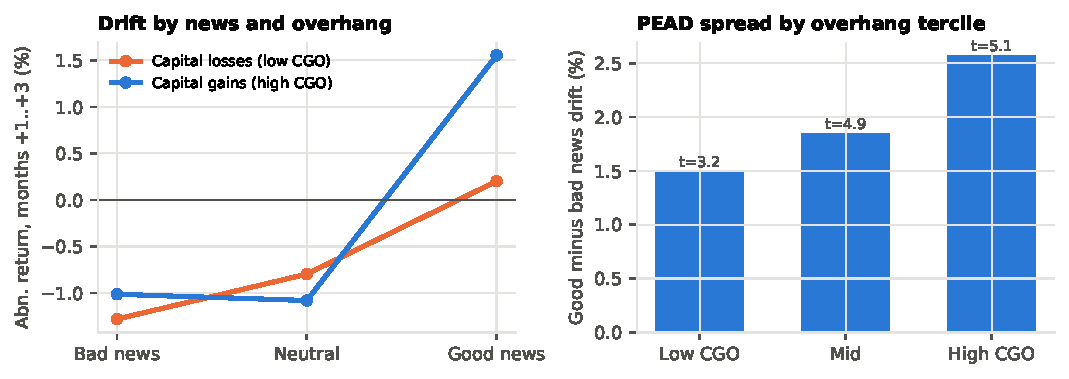
\includegraphics[width=0.97\textwidth]{results/fig_main.pdf}\end{center}

\begin{center}\small
\begin{tabular}{lcc}
\toprule
Test (months $+1$ to $+3$, \%) & Estimate & $t$\\
\midrule
PEAD spread (good minus bad news), low / mid / high CGO & 1.48 / 1.84 / 2.57 & 3.3 / 4.9 / 5.1\\
High-CGO minus low-CGO PEAD spread & 1.09 & 2.0\\
\quad good news: gains minus losses & 1.35 & 1.8\\
\quad bad news: losses minus gains & $-0.27$ & $-0.4$\\
Frazzini aligned (good/gains minus bad/losses) vs misaligned & 2.84 vs 1.21 & 3.9 vs 1.5\\
\midrule
FM, SUE $\times$ CGO interaction: drift / announcement month & 0.04 / 0.08 & 0.2 / 0.8\\
FM, CGO main effect in the announcement month & $-0.67$ & $-4.3$\\
\bottomrule
\end{tabular}\\[2pt]
{\footnotesize FM slopes are per 1 SD, with size, B/M, momentum and turnover controls.}
\end{center}

\sect{Findings}
\begin{itemize}
\item \textbf{Drift is larger when shareholders sit on gains, but only on the upside.} The good-minus-bad-news drift
  rises from 1.5\% to 2.6\% over three months from the lowest to the highest CGO tercile ($t=2.0$ for the
  difference). The increase comes from good news among stocks with gains, consistent with disposition selling of
  winners dampening the initial reaction. Bad news among losers does not drift more, unlike in Frazzini.
\item \textbf{The continuous interaction is weak.} In Fama--MacBeth regressions the SUE $\times$ CGO term is
  insignificant, so the effect is concentrated in the tails rather than linear.
\item \textbf{The overhang itself predicts announcement-month returns.} Stocks with gains underperform in the
  announcement month by 0.67\% per SD ($t=-4.3$), consistent with disposition selling as attention spikes.
\item \textbf{The overhang does not explain the streak result.} Positive streaks carry slightly more gains, but
  adding CGO and SUE $\times$ CGO leaves the streak interaction unchanged. In this simple specification (SRW SUE,
  three-month drift) the streak interaction is itself insignificant, unlike in the paper's baseline, so this check
  should be redone inside the paper's own Fama--MacBeth framework.
\end{itemize}

\sect{Assessment and next steps}
A credible ``China version of Frazzini'' with a twist: the asymmetry (winners only). Short-sale constraints may
explain why bad news on losers does not drift. Next: (i) daily-volume reference prices for precision;
(ii) test the asymmetry against shortable versus non-shortable stocks (2010 margin-trading pilot list); (iii)
compare with the 52-week-high anchor (George and Hwang, 2004) to separate disposition from anchoring. Moderate
novelty; best used as a mechanism or robustness section rather than a standalone Q1 paper.
\end{document}
